\documentclass[a4paper, 12pt]{article}
\usepackage{amsmath}
\usepackage{amssymb}
\usepackage{dsfont}
\usepackage[left=1.5cm, right=1.5cm, bottom=2cm, top=2cm]{geometry}
\usepackage{graphicx}
\usepackage{hyperref}
\usepackage[utf8]{inputenc}
\usepackage{microtype}
\usepackage{natbib}
\usepackage{tikz}
\newcommand{\given}{\,|\,}

\title{}
\author{}
\date{}

\begin{document}
\maketitle

%\abstract{}

% Need this after the abstract
\setlength{\parindent}{0pt}
\setlength{\parskip}{8pt}

Let $\boldsymbol{x}_i \in \mathcal{X}$ be the microscopic details of the
history of star
$i$ in the universe over time $t$. There is a region of $\mathcal{X}$ indicating
that life exists at some point during the history.
Call that region $L$. There is another region
$O$ indicating that conscious observers exist at some point during the history.
Conscious observers have some memories that may or may not equal mine.
Call that region $O$. It is a subset of
$L$. Within $L$, there is a tiny subregion $B$ indicating that Brendon exists.

Now consider the probability that a trajectory $\boldsymbol{x}(t)$ is inside
$B$. This is three subsets in. So we can factorise it using the chain-product
rule.
\begin{align}
P(B) &= P(L)P(O \given L)P(B \given O).
\end{align}
We can parameterise it this way:
\begin{align}
P(B) &= P(L)P(O \given L)P(B \given O) \\
     &= \theta\phi\epsilon,
\end{align}
But this leads to extreme self indication.

What if I set the marginal probability of $B$ to be $\epsilon$, rather than
the conditional probability. Then we have
\begin{align}
\epsilon &= \theta\phi P(B \given O) \\
\therefore
P(B \given O) &= \frac{\epsilon}{\theta\phi}.
\end{align}
This would completely cancel any indication factors but seems wrong.


, including life (if any) and conscious beings (if any)
that arise around it. Presumably $\boldsymbol{x}_i$ is a point in a very high
dimensional space $\mathcal{X}$, perhaps analogous to a phase space in
statistical mechanics.
Define the following proposition:
\begin{align}
L\textnormal{:}\quad\textnormal{Life arises around star}~i. 
\end{align}
This defines $L$ as a subset of the space of possible micro-histories of a star.
We can define a smaller subset for at least one conscious observer,
whose details we currently omit. This subset relates to any conscious observer
regardless of the contents of their consciousness:
\begin{align}
O\textnormal{:}
\quad\textnormal{At least one conscious observer arises around star}~i. 
\end{align}
Of course, $O$ implies $L$, so we have $O \subset L \subset \mathcal{X}$.
Finally, we define the narrowest possible subset of $\mathcal{X}$ that we
will consider, which is
\begin{align}
B\textnormal{:}
\quad\textnormal{Brendon Brewer's memory state is instantiated around star}~i. 
\end{align}
$B$ includes the fact of being at $t=13.8$ Gyr, and being around a G star.
So far, all propositions about $\boldsymbol{x}_i$ have been nested, i.e.,
$B \implies O \implies L$.
Hypothetical alternative observers around M stars are within $O$ (and thus
also within $L$), but are mutually exclusive with $B$. We will call the
subset with M star observers $O_M$.

\begin{figure}
\centering
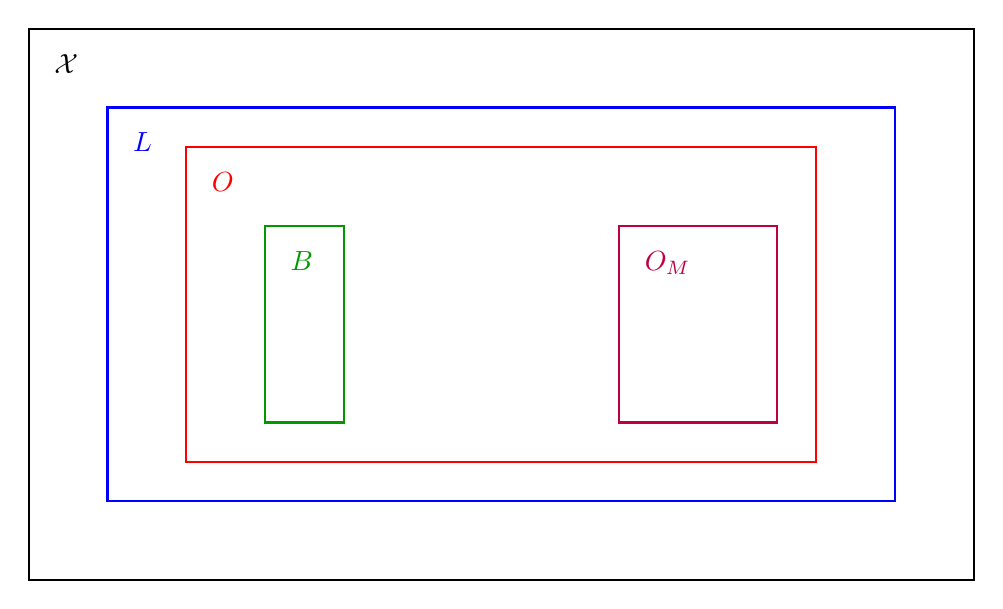
\begin{tikzpicture}[scale=1]

  % Ambient space X
  \draw[thick] (0,0) rectangle (12,7);
  \node[anchor=north west] at (0.2,6.8) {$\mathcal{X}$};

  % L subset
  \draw[thick,blue] (1,1) rectangle (11,6);
  \node[anchor=north west,blue] at (1.2,5.8) {$L$};

  % O subset
  \draw[thick,red] (2,1.5) rectangle (10,5.5);
  \node[anchor=north west,red] at (2.2,5.3) {$O$};

  % B subset (your microhistory)
  \draw[thick,green!60!black] (3,2) rectangle (4.0,4.5);
  \node[anchor=north west,green!60!black] at (3.2,4.3) {$B$};

  % O_M subset (M-star observers)
  \draw[thick,purple] (7.5,2) rectangle (9.5,4.5);
  \node[anchor=north west,purple] at (7.7,4.3) {$O_M$};

\end{tikzpicture}
\caption{The full space $\mathcal{X}$ of possible micro-histories of a given
star (star $i$), and various subsets of the space. Volumes are definitely
not to scale!\label{fig:sets}}
\end{figure}

\section*{An Individual Star}
Consider an individual star which may be type $G$ or $M$.
Suppose its microhistory satisfies $L$ with probability $\theta_G$ if it is
a G star, or with probability $\theta_M$ if it is an M star.
Conditional on being within $L$, it develops at least one observer with
probability $\phi_G$ if it is a G star or $\phi_M$ if it is an M star.
Overall, we have the product rule along chains (which resembles the Drake
equation) giving
\begin{align}
P(B \given \boldsymbol{\theta}) &= \theta_G \phi_G \epsilon
\end{align}
for a G star or
\begin{align}
P(B \given \boldsymbol{\theta}) &= 0
\end{align}
for an M star.
Therefore the probability of $\neg B$ for an individual star is
\begin{align}
P(\neg B \given \boldsymbol{\theta}) &= 1 - \theta_G \phi_G \epsilon
\end{align}
for a G star or 1 for an M star.

Bad SIA-type likelihood:
The probability of no occurrence of Brendon anywhere is
\begin{align}
P(\textnormal{no Brendon anywhere} \given \boldsymbol{\theta})
    &= \left(1 - \theta_G \phi_G \epsilon\right)^{N_G}.
\end{align}
Thus, the probability of at least one Brendon is
\begin{align}
P(\textnormal{at least one Brendon} \given \boldsymbol{\theta})
    &= 1 - \left(1 - \theta_G \phi_G \epsilon\right)^{N_G}.
\end{align}
We will work in the regime where $\theta_G\phi_G\epsilon$ is tiny,
giving an approximation
\begin{align}
P(\textnormal{at least one Brendon} \given \boldsymbol{\theta})
    &\approx N_G \theta_G \phi_G \epsilon.
\end{align}
This is the bad FNC likelihood.

Good (?) likelihood:
The probability of a consciousness anywhere is
\begin{align}
P(\textnormal{at least one consciousness} \given \boldsymbol{\theta})
    &= 1 - \left(1 - \theta_G \phi_G \right)^{N_G}
           \left(1 - \theta_M \phi_M \right)^{N_M}.
\end{align}
Given that there is a consciousness anywhere, assume a probability distribution
$p(n_G, n_M \given \boldsymbol{\theta})$ for the number of them.
\begin{align}
P(\textnormal{at least one consciousness}, n \given \boldsymbol{\theta})
    &= \left[1 - \left(1 - \theta_G \phi_G \right)^{N_G}
           \left(1 - \theta_M \phi_M \right)^{N_M}\right]p(n_G, n_M \given \boldsymbol{\theta}).
\end{align}


\section*{Components Analogy}



\end{document}

